\documentclass[final,hyperref={pdfpagelabels=false},fleqn]{beamer}
\mode<presentation>
{
  \usetheme{Berlin}
  % \usetheme{Dreuw}
  % \usetheme{Singapore}
  % \usetheme{Boadilla}
  % \usetheme{Copenhagen}
  % \usetheme{Madrid}
}
\usepackage{times}
\usepackage{amsmath}
\usepackage{amsfonts}
\usepackage{amsmath}
\usepackage{amssymb}
% \usepackage[fleqn]{amsmath}
% \usepackage{amsthm}
% \usepackage{amssymb}
% \usepackage{latexsym}
\boldmath
\usepackage{exscale}
\usepackage[english]{babel}
\usepackage[latin1]{inputenc}
\usepackage[orientation=portrait,size=a1]{beamerposter}
% \usepackage[orientation=portrait,size=a0,scale=1.4,debug]{beamerposter}
\usepackage{ragged2e} 
\renewcommand\baselinestretch{1.08} 

%%%%%%%%%%%%%%%%%%%%%%%%%%%%%%%%%%%%%%%%%%%%%%%%%%%%%%%%%%%%%%%%%%%%%%%%%%%%%%%%% 5
\title{Estimating the force computation error in inhomogeneous and correlated molecular systems}
\author{Han Wang\inst{1}, Christof Sch\"utte\inst{1}, Pingwen Zhang\inst{2}}
\institute[]{ \footnotesize
  \inst{1} Institute for Mathematics, Freie Universit\"at Berlin, Germany\\
  \inst{2} LMAM and School of Mathematical Sciences, Peking University, P.R. China  
}
% \date{Jul. 31th, 2007}
%  \RequirePackage{tangocolors}
%  \setbeamercolor{headline}{fg=black,bg=tagray}

%%%%%%%%%%%%%%%%%%%%%%%%%%%%%%%%%%%%%%%%%%%%%%%%%%%%%%%%%%%%%%%%%%%%%%%%%%%%%%%%% 5

\begin{document}

\newcommand{\redc}[1]{{\color{red} #1}}
\newcommand{\bluec}[1]{{\color{blue} #1}}
\renewcommand{\v}[1]{\textbf{\textit{#1}}}
\renewcommand{\d}[1]{\textrm{#1}}

\begin{frame}{}
  % \vskip -1cm
  \begin{beamercolorbox}[wd=\paperwidth]{headline}
    \begin{columns}[T]
      \begin{column}{.18\paperwidth}
        \begin{center}
          \hspace{4ex}\includegraphics[width=.6\linewidth]{logo/500px-Seal_of_Free_University_of_Berlin.png}
        \end{center}
      \end{column}
      \begin{column}{.6\paperwidth}
        \vskip1ex
          % \raggedleft
        \centering
        \usebeamercolor{title in headline}{\color{fg}\textbf{\Large{\inserttitle}}\\[1ex]}
        \usebeamercolor{author in headline}{\color{fg}\large{\insertauthor}\\[1ex]}
        \usebeamercolor{institute in headline}{\color{fg}\large{\insertinstitute}\\[1ex]}     
        \vskip4ex
      \end{column}
      \begin{column}{.18\paperwidth}
        \begin{center}
          \hspace{4ex}
\includegraphics[width=.61\linewidth]{logo/pku.png}
          % \vspace*{-1em}
          % \hspace{-2ex}\includegraphics[width=.4\linewidth]{logo/unilogo}\\
          % \vspace*{0.5em}
          % \hspace{-2ex}\includegraphics[width=.6\linewidth]{logo/Logo_ICP_T_V2}
          % \vfill
        \end{center}
      \end{column}
    \end{columns}
  \end{beamercolorbox}

  
  \vfill
  % \vspace{-1cm}
  \begin{columns}[t]
    \begin{column}{.48\linewidth}
      \vfill
      \begin{block}{\large Abstract}
        \vspace{1ex}
        \begin{minipage}[c]{.975\linewidth}
          We derive the error estimate of force computation (both short-range
          and long-range interactions) in inhomogeneous and correlated systems.
          The root mean squared (RMS) error is proved to be composed of
          three additive parts: the homogeneity error, the inhomogeneity error
          and the correlation error. Numerical methods are proposed to
          estimate these errors at an acceptable computational cost, namely
          $\mathcal O(N\log N)$. The unphysical artifacts of the force error
          are also discussed by examples.
        \end{minipage}
      \end{block}
      \vspace{.3ex}
      \begin{block}{Motivations}
        \textbf{Why study the force calculation:}
        \begin{itemize}
        \item Computationally intensive: \redc{$ \sim 90 \%$}.
        \item One of the main sources of the \redc{``error''}.
        \item Inhomogeneity: \redc{unphysical artifacts}.
        \item Correlation: complexity of error estimate.
        \end{itemize}
        \textbf{What can we do with the error estimates:}
        \begin{itemize}
        \item Understanding \& correcting
          the unphysical artifacts, quantitatively.
        \item Correction to \redc{force, energy, pressure, etc.}
        \item Boost the \redc{accuracy \& efficiency} of simulation automatically.
        \end{itemize}
      \end{block}
      \vspace{.3ex}
      \begin{block}{Theory}
        Let a periodic molecular system be composed by $N$ charged
        particles located at $\v r_1, \v r_2, \cdots, \v r_N$ with
        charges $q_1, q_2, \cdots, q_N$, respectively. If the error
        force of a testing particle located at $\v r$ with charge $q$
        is: \bluec{
          \begin{align}\label{eqn:thm-error-force}
            \Delta \v F(\v r) =
            q\sum_{j=1}^N\,q_j \v K(\v r, \v r_j),
          \end{align}}
        then the mean error force is estimated by
        \bluec{
          \begin{align}
            \langle\Delta\v F(\v r)\rangle
            =
            q\int_{\mathbb R^3}\v K(\v r , \v r')\,\rho_q(\v r')\,\d d\v r'.
          \end{align}
        }
        The RMS error is estimated by:
        \bluec{
          \begin{align} 
            \langle\vert\Delta\v F(\v r)\vert^2\rangle
            = 
            \redc{\mathcal E^2_{\textrm{homo}}(\v r)} +
            % \langle\Delta\v F(\v r)\,\rangle^2 +
            \redc{\mathcal E^2_{\textrm{inhomo}}(\v r)} +
            \redc{\mathcal E_{\textrm{correlation}}(\v r)},
          \end{align}
        }
        with\bluec{
          \begin{align}
            &{\mathcal E^2_{\textrm{homo}}(\v r)}
            = \,
            q^2\int_{\mathbb R^3}\vert\v K(\v r, \v r')\vert^2\rho_{q^2}(\v r')\,\d d\v r', \\
            &{\mathcal E^2_{\textrm{inhomo}}(\v r)}
            = \,
            q^2\bigg[\int_{\mathbb R^3}\v K(\v r, \v r')\rho_q(\v r')\,\d d\v r'\,\bigg]^2
            \redc{ = \langle\Delta\v F(\v r)\,\rangle^2},
            \\
            &{\mathcal E_{\textrm{correlation}}(\v r)}
            =\,
            q^2\int_{\mathbb R^3\times\mathbb R^3}\v K(\v r, \v r')\cdot\v K(\v r, \v r'')\,C_{q^2}(\v r', \v r'')\,\d d\v r'\d d\v r''.
          \end{align}}
        When the kernel has a convolution form:
        \bluec{
          \begin{align}
            \v K(\v r,\v r') = \v K(\v r- \v r'),
          \end{align}
        }
        the computational cost of the homogeneity error and inhomogeneity error estimates are
        \redc{$\mathcal O(N\log N)$}, while the correlation error
        is \bluec{$\mathcal O(N^2\log N)$}. Nearest neighbor approximation: \redc{$\mathcal O(N\log N)$}.        
        % First neighbor approximation of the correlation error, take water for example:
        % \bluec{
        %   \begin{align}\nonumber
        %     \mathcal E_{\textrm{correlation}}(\v r)
        %     =&\,
        %     q^2
        %     \int_{\mathbb R^3}
        %     \v K(\v r - \v r')\cdot
        %     (\hat T_{\textrm{O}}\hat{\v K})^{\vee}(\v r - \v r')
        %     \,\rho_{\textrm{O}}(\v r')
        %     \,\d d\v r' \\\label{eqn:c-error-water}
        %     & \,+
        %     q^2
        %     \int_{\mathbb R^3}
        %     \v K(\v r - \v r')\cdot
        %     (\hat T_{\textrm{H}}\hat{\v K})^{\vee}(\v r - \v r')
        %     \,\rho_{\textrm{H}}(\v r')
        %     \,\d d\v r',
        %   \end{align}}
        % where
        % \bluec{
        %   \begin{align}
        %     \hat T_{\textrm{O}}(\v m)
        %     &= 
        %     2\langle
        %     q_{\textrm{H}}\,e^{2\pi i\v m\cdot\v s_{\textrm{O}}}
        %     \rangle,\\
        %     \hat T_{\textrm{H}}(\v m)
        %     &= 
        %     \langle
        %     q_{\textrm{O}}\,e^{-2\pi i\v m\cdot\v s_{\textrm{O}}} +
        %     q_{\textrm{H}}\,e^{2\pi i\v m\cdot\v s_{\textrm{H}}}
        %     \rangle.
        %   \end{align}}
        % The correlation error can be approximately calculated at the cost of
        % \redc{$\mathcal O(N\log N)$}.
      \end{block}
      \vspace{.3ex}
      \begin{block}{Long-range force \& pressure correction}
        The calculated force can be corrected by the mean error force:
        \bluec{
          \begin{align}\label{eqn:define-fcorr}
            \v F_{\textrm{corr}}(\v r) = {\v F}_{\textrm{orig}}(\v r) + \langle\Delta\v F(\v r)\rangle.
          \end{align}}
        The new mean error force varnishes:
        \bluec{
          \begin{align}\label{eqn:mean-fcorr}
            \langle\Delta\v F_{\textrm{corr}}(\v r)\rangle
            =
            \big\langle\,
            \v F(\v r) - {\v F}_{\textrm{orig}}(\v r) - \langle\Delta\v F(\v r)\rangle\,
            \big\rangle \redc{= 0}.
          \end{align}}
        The mean square error is given by
        \bluec{
          \begin{align} \nonumber
            \langle\vert\Delta\v F_{\textrm{corr}}(\v r)\vert^2\rangle
            & =
            \redc{\mathcal E^2_{\textrm{homo}}(\v r)} +
            \redc{\mathcal E_{\textrm{correlation}}(\v r)}.
          \end{align}}
        No inhomogeneity error any more! Pressure correction:
        \bluec{
          \begin{align} 
            \v P_{\textrm{corr}}
            & = \int_{\mathbb R^3\times\mathbb R^3}
            \frac1{2V}[\v r\otimes\v K](\v r' - \v r'')
            \rho(\v r') \rho(\v r'') 
            \d d\v r'\d d\v r'' 
          \end{align}}          
      \end{block}
    \end{column}
    \begin{column}{.48\linewidth}
      \begin{block}{Adaptive cut-off}
        Use larger cut-off radius for interfacial regions, while use smaller
        cut-off radius for bulk regions. The error estimate guarantee the error
        is uniformly distributed.
      \end{block}
      \begin{block}{Short-range example}
        \begin{figure}
          \centering
          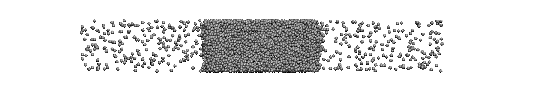
\includegraphics[width=0.85\textwidth]{figs/t0.85-n16000-rc07.5uni/confout-02.eps}\\
          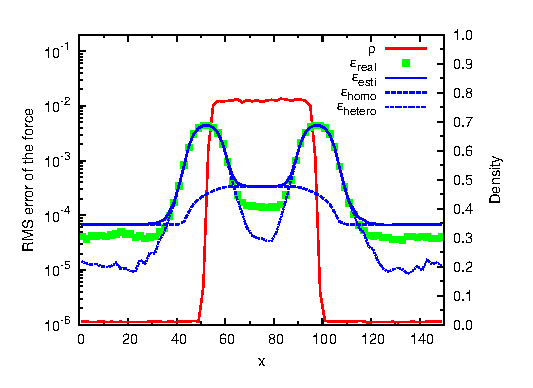
\includegraphics[width=0.85\textwidth]{figs/t0.85-n16000-rc07.5uni/error-uniform.eps}
          \caption{An inhomogeneous system: liquid-vapor equilibrium of Lennard-Jones particles.
            $T^\ast = 0.85$.}
        \end{figure}
      \end{block}
      \begin{block}{Convergence check with respect to cut-off}
        \begin{figure}
          \centering
          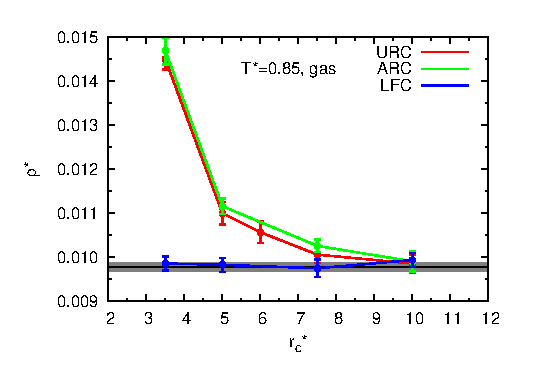
\includegraphics[width=0.85\textwidth]{figs/converge.new/t0p85-gas.eps}\\
          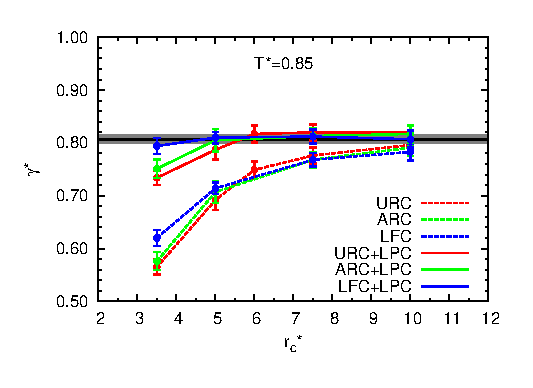
\includegraphics[width=0.85\textwidth]{figs/converge.new/tension-t0p85.eps} 
          \caption{Convergence check of equilibrium vapor density and
            surface tension with respect to cut-off radius.
            Reference (black line with gray region denoting the
            uncertainty) was obtained at cut-off of $r^\ast_c =
            13$. URC: uniform cut-off, ARC: the adaptive cut-off and
            LFC: the long-range force correction, LPC: long-range
            pressure correction. }
        \end{figure}
        % \begin{figure}
        %   \centering
        %   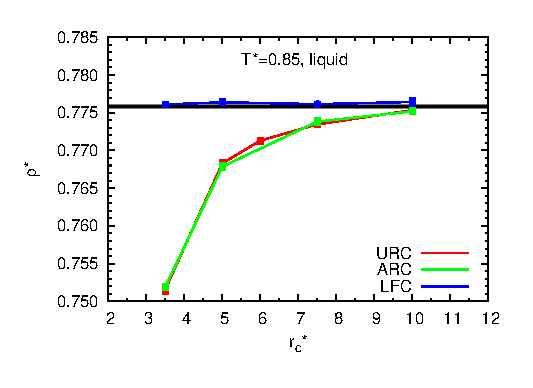
\includegraphics[width=0.85\textwidth]{figs/converge.new/t0p85-liquid.eps} 
        % \end{figure}
      \end{block}
    \end{column}
    % \begin{column}{.32\linewidth}
    % \end{column}
  \end{columns}
  \vfill
  \end{frame}
\end{document}


%%%%%%%%%%%%%%%%%%%%%%%%%%%%%%%%%%%%%%%%%%%%%%%%%%%%%%%%%%%%%%%%%%%%%%%%%%%%%%%%%%%%%%%%%%%%%%%%%%%%
%%% Local Variables: 
%%% mode: latex
%%% TeX-PDF-mode: t
%%% End:
